%===================================== CHAP 2 =================================

\chapter{Literature Review}

%Web and experience, enric pliaza, ralph bergmann, CBR stuff cooking recepies

%Mining stories from web
\section{Related work}
Discuss other articles that touch on the same subject

\subsection{SMILA} \label{smila}

\begin{figure}[h]
\caption{An overall overview of the SMILA architecture}
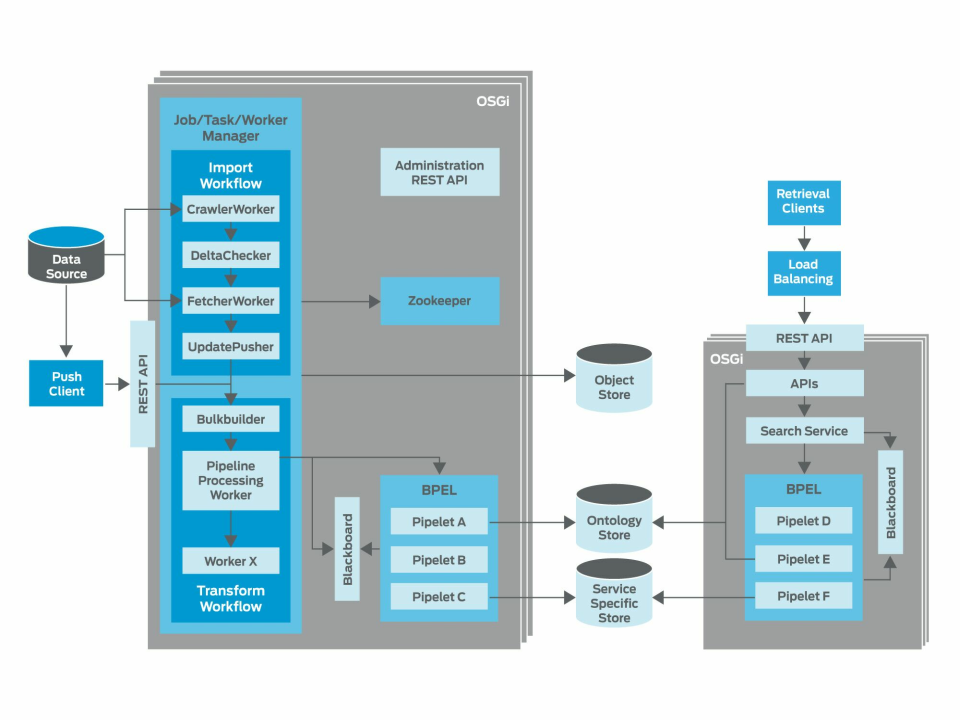
\includegraphics[width=\textwidth]{SMILA_Architecture}
\end{figure}

%%fix sånn abbrevation for SMILA

%%når jeg snakker om mine erfaringer med smila gjør jeg det i implementation.

%%Skriv om dette til å passe til sin nye kontekst
In the early stages of the project, an existing project called SMILA was explored. SMILA crawls the web to extract information and then stores the information in an index. It has a REST API to control the system and for searching the index. The SMILA architecture is also based on the pipeline architecture containing the following processes jobs, crawling, storage, indexing and querying. With SMILA being very complex, it gains asynchronicity as its biggest benefit from the pipeline architecture. The SMILA pipeline also allows custom made pipelets to be inserted into the pipeline. A pipelet is a sub process inside a pipeline. By creating pipelets, the behaviour of SMILA could be tailored into extracting the relevant information from Wikipedia.

By only writing pipelets and then make SMILA use them when crawling Wikipedia, the project could concentrate the effort on identifying and indexing the examples. Unfortunately SMILA is an old and complex system, and is rarely updated anymore. When problems running SMILA appeared, it was quite troublesome to understand why and fix the issue. This ironically lead to all the effort in the starting phase being used on making SMILA run properly, instead of looking into the characteristics of examples. 

\section{Techniques}

\subsection{Pipeline} \label{pipeline}
Describe a software pipeline. Advantages and stuff.\\
How should i use references for this?


\cleardoublepage